\section{OpenCL}

Cette section est basée sur les informations consultées dans le livre 
\textit{OpenCL Programming Guide}\autocite{openclguide}. 

Dans les prochaines sections, il faut comprendre que \texttt{OpenCL} travaille 
avec une queue d'exécution et que l'ensemble des opérations permettant de l'appeller 
sont des événements ajoutés à cette queue.

\subsection{Introduction à l'OpenCL}

\texttt{OpenCL} est une couche d'abstraction des composants matériels. 
Il permet de s'appuyer sur des GPUs et CPUs pour exécuter des programmes dits 
\texttt{Kernels}. On s'intéresse ici au \texttt{GPGPU} 
\textit{(general-purpose computing on graphics processing units)}. Afin d'utiliser 
nos composants de manière efficace, la parallélisation est primordiale. On retrouve 
ainsi deux grands types de parallélisation:
\begin{itemize}
    \item \textbf{\textit{data parallelisation}}: s'utilise lorsqu'on cherche à traiter
        différentes parties des données avec une même opération
    \item \textbf{\textit{task parallelisation}}: s'utilise si on cherche à exécuter des 
        kernels en parallèle
\end{itemize}

\subsection{Modèle d'exécution \textit{(execution model)}}

Afin de pouvoir s'intéresser à comment mettre en oeuvre la parallélisation, il faut 
d'abord s'intéresser au modèle d'exécution d'\texttt{OpenCL}. Une application 
\texttt{OpenCL} est constituée de deux parties: un programme hôte et des kernels.

Le programme hôte permet d'interfacer avec les composants et d'ainsi y exécuter 
les kernels définis pour cette application (figure~\ref{fig:host_device_interaction}).
Afin de lancer un kernel, il faut lui passer un tuple de dimensions sur lequel il va 
``itérer'' afin d'appliquer le code aux données: on l'appelle le 
\textbf{\textit{global NDRange}} \textit{(N dimensions range)} qu'on notera $G$.
Lorsqu'un kernel est lancé par le programme hôte, $X_g$ \textbf{\textit{work items}} tel que 
${\displaystyle X_g = \prod_{i=0}^{N}G[i]}$ sont crées et exécutent chacun le même
kernel concurrement. Pour pouvoir paralléliser l'exécution du kernel il faut 
créer plusieurs \textbf{\textit{work groups}} (figure~\ref{fig:execution_model}).

\begin{figure}[h]
    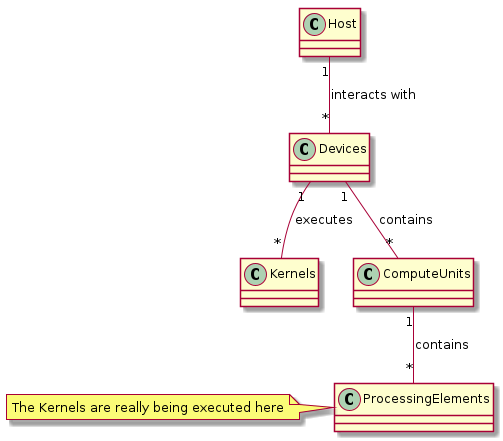
\includegraphics[width=0.6\textwidth]{../../resources/host_device_relationship.png}
    \caption{Interaction entre les différents composants définis d'OpenCL}
    \label{fig:host_device_interaction}
\end{figure}

On suppose ici que $G$ est composé de deux dimensions tel que $G = (G_x, G_y)$.
Alors, à chaque \textit{work item} on associe une coordonnée unique $g = (g_x, g_y)$ tel que 
$g_x \in [0..G_x-1]$ et $g_y \in [0..G_y-1]$ dit identifiant global. 
Ceux-ci sont alors groupés dans des
\textit{work groups} qui eux peuvent s'exécuter parallèlement pour autant de 
\textbf{\textit{compute units}} (figure~\ref{fig:host_device_interaction}) existants. 
Le nombre d'éléments crées par \textit{work group} 
est défini par le \textbf{\textit{local NDRange}} qu'on notera $L = (L_x, L_y)$. 
Grâce à $L$ on obtient le \textit{NDRange} des \textit{work groups} qu'on notera $W = (W_x, W_y)$ 
tel que 
$$L_x = G_x / W_x$$ 
$$L_y = G_y / W_y$$ 
Cela a pour conséquence que $G_x \bmod W_x = 0$ et 
$G_y \bmod W_y = 0$. Cela a aussi pour conséquence que le nombre d'éléments $X_w$ dans 
un \textit{work group} est ${\displaystyle X_w = \prod_{i=0}^{N}L[i]}$ 
(figure~\ref{fig:execution_model}). 

\begin{figure}[h]
\begin{center}
    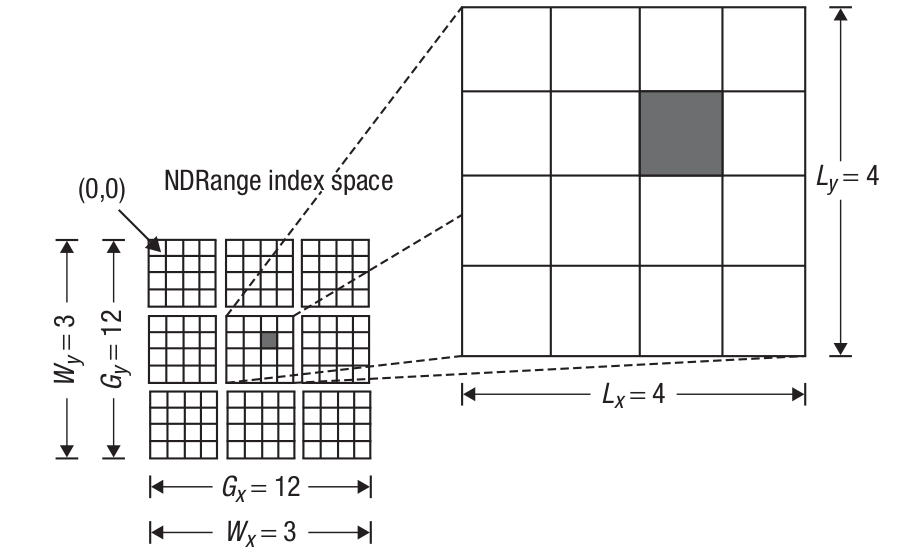
\includegraphics[width=0.9\textwidth]{../../resources/execution_model.png}
    \caption{Modèle d'exécution d'OpenCL avec le détail des \textit{work groups} 
    et \textit{work items}}
    \label{fig:execution_model}
\end{center}
\end{figure}

Ces identifiants sont importants car ils nous permettent de comprendre comment parcourir 
l'ensemble de nos éléments dans les différentes régions de la mémoire vues dans la 
prochaine sous-section.

\subsubsection{Modèle de mémoire \textit{(memory model)}}\label{sec:memory_model}

Le modèle de mémoire se base sur des \textit{memory objects}, il en existe deux types:
\begin{itemize}
    \item \textbf{\textit{buffer objects}}: block continue de données de n'importe quels types 
        (il est possible de passer des structures)
    \item \textit{image objects}: objet spécialisé pour le traitement d'images
\end{itemize}

Avant de voir les interactions hôte-composant, on doit d'abord s'intéresser aux 
5 distinctes \textbf{régions de mémoire} (Figure~\ref{fig:memory_model}):
\begin{itemize}
    \item \textbf{\textit{host memory}}: la mémoire de l'hôte disponible uniquement 
        pour celui-ci
    \item \textbf{\textit{global memory}}: la mémoire globale disponible à tous les 
        \textit{work items} en écriture et lecture
    \item \textbf{\textit{constant memory}}: la mémoire constante disponible à tous 
        les \textit{work items} uniquement en lecture
    \item \textbf{\textit{local memory}}: la mémoire locale disponible à tous les 
        \textit{work items} d'un même \textit{work group}
    \item \textbf{\textit{private memory}}: la mémoire privée disponible uniquement 
        au \textit{work item} qui la déclare
\end{itemize}

Pour avoir accès aux données de l'hôte, il nous faut soit les copier ou les mapper 
sur le composant utilisé. Ces interactions sont définies par l'hôte. On passe par 
des buffers afin de pouvoir les rendre accessible au kernel. Ces opérations peuvent 
êtres bloquantes, on s'assure alors que la donnée est prête, ou non bloquantes 
alors le programme hôte reprend dès que l'événement a été rajouté à la queue. 
Ces buffers seront accessibles depuis la mémoire globale après avoir été passés en
arguments (voir Section~\ref{sec:execution_kernel}).

\begin{figure}[h]
\begin{center}
    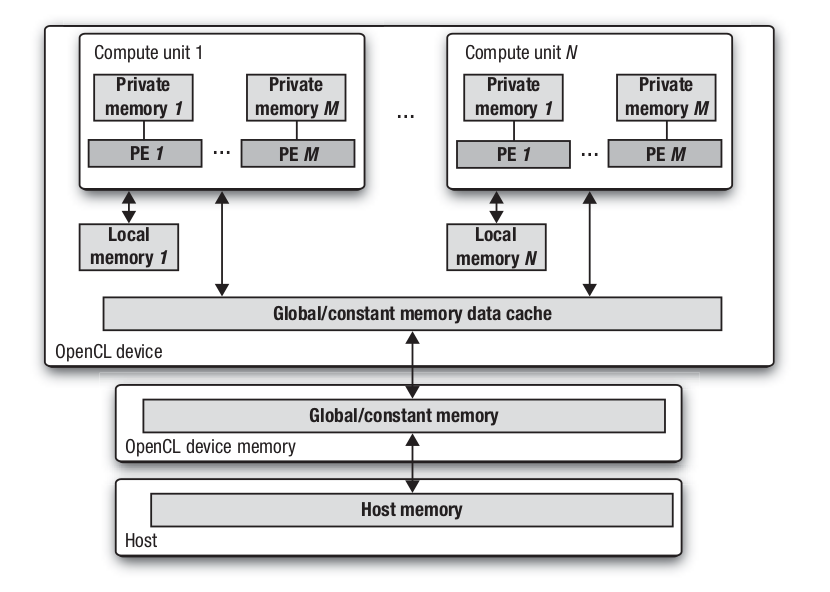
\includegraphics[width=0.9\textwidth]{../../resources/memory_model.png}
    \caption{Modèle de mémoire d'OpenCL}
    \label{fig:memory_model}
\end{center}
\end{figure}

\subsubsection{Le Kernel}

Le kernel s'écrit en \textit{\textbf{OpenCL C}} qui est un dérivé du C99. 
Cependant, des fonctionnalités souvent utilisées en C y ont été retirées:
\begin{itemize}
    \item la récursivité
    \item les pointeurs de fonctions
    \item l'allocation dynamique
    \item les \textit{bit fields}
\end{itemize}

Des types spéciaux y ont été rajoutés tel que \textit{float4} qui permet de 
travailler directement sur des vecteurs d'ici 4 éléments. Ces types ont été 
ajoutés afin de pouvoir exploiter du parallélisme de données.
On retrouve aussi l'ajout de fonctions de synchronisation tel que \textit{barrier}.

Des exemples de kernel sont disponibles plus loin (voir Sections~\ref{sec:pyopencl}
et~\ref{sec:matrixmultiplication}).

\subsection{Installation d'OpenCL}

L'installation d'\texttt{OpenCL} passe par deux étapes:
\begin{itemize}
    \item l'installation des \textit{headers}: c’est l’API qui est définie 
        par \texttt{Khronos Group}
    \item l'installation des \textit{runtimes}: c’est l’implémentation qui est 
        définie par le vendeur du GPU (\texttt{Nvidia}, \texttt{AMD} ou 
        \texttt{Intel})
\end{itemize}

\subsubsection{L'installation des \textit{headers} sous Linux}

Cette étape passe par une ligne de commande:
\begin{lstlisting}
   sudo apt install opencl-headers
\end{lstlisting}

\subsubsection{L'installation des \textit{runtimes} d'Intel sous Linux}

Cette étape contient deux sous parties. On va d'abord installer le 
\textit{compute runtime} qui va nous permettre d'exécuter du code 
\texttt{OpenCL} sur notre machine. Les premiers paquets à installer se trouvent 
sur le github d'\texttt{Intel} \autocite{intelgit}. Le processus d'installation 
décrit ci-dessous peut aussi être trouvé à ce lien. 
\begin{lstlisting}[language=sh]
mkdir neo
cd neo
# do not copy paste, it might not be the most recent version
wget https://github.com/intel/compute-runtime/releases/download/19.14.12751/intel-gmmlib_19.1.1_amd64.deb
wget https://github.com/intel/compute-runtime/releases/download/19.14.12751/intel-igc-core_19.11.1622_amd64.deb
wget https://github.com/intel/compute-runtime/releases/download/19.14.12751/intel-igc-opencl_19.11.1622_amd64.deb
wget https://github.com/intel/compute-runtime/releases/download/19.14.12751/intel-opencl_19.14.12751_amd64.deb
wget https://github.com/intel/compute-runtime/releases/download/19.14.12751/intel-ocloc_19.14.12751_amd64.deb
# use apt install to ensure any missing dependencies will be installed
sudo apt install ./*deb         
\end{lstlisting}
\vspace{10pt}
On va maintenant installer les libraries qui vont nous permettre de compiler 
le code. Pour cela il nous faut télécharger l'archive au niveau des 
\textit{OpenCL drivers} d'\texttt{Intel} dans la section 
\textit{``Intel CPU Runtime for OpenCL''} \autocite{inteldrivers}. 
Ensuite, on installe ces derniers avant de configurer la liaison dynamique 
de la librarie \autocite{streamhpc}. Le processus est montré ci-dessous.
\begin{lstlisting}[language=sh]
# the downloaded file might not have the same name and paths may vary
tar -xvf l_opencl_p_18.1.0.015.tgz
cd l_opencl_p_18.1.0.015/rpm
# requires alien and libnuma1 - converts everything to deb packages
alien *.rpm
# use apt install to ensure any missing dependencies will be installed
sudo apt install ./*deb
# makes directories for vendors
sudo mkdir -p /usr/lib/OpenCL/vendors/
sudo mv /opt/intel /usr/lib/OpenCL/vendors/
sudo cp /usr/lib/x86_64-linux-gnu/libOpenCL.so /usr/lib/OpenCL/vendors/intel/libOpenCL.so
# configure dynamic linking
sudo echo "/usr/lib/OpenCL/vendors/intel" > /etc/ld.so.conf.d/opencl-vendor-intel.conf
sudo ldconfig
\end{lstlisting}

\subsubsection{Test de l'installation}

Un test simple de l'installation peut se faire avec la commande \textit{clinfo} 
qui permet de lister un ensemble d'information sur les composants supportant 
\texttt{OpenCL} disponible sur la machine.
